\documentclass{report}
\def\atitle{Development of a Control System Using a Raspberry Pi}
\def\theauthor{Christopher Boyle}

% Imports
\usepackage{graphicx}
\usepackage[a4paper]{geometry}
\usepackage{fancyhdr}
\usepackage[english]{babel}
\usepackage{etoolbox}
\usepackage{url}
\usepackage[hidelinks]{hyperref}
%\usepackage{titlesec}

% Unused packages
%\usepackage{placeins}
%\usepackage{fancyref}
%\usepackage[comma,authoryear]{natbib}
%\usepackage{lipsum}

% Settings
\geometry{top=2cm, bottom=2cm, left=0cm, right=0cm}
\patchcmd{\chapter}{\thispagestyle{plain}}{\thispagestyle{plain}}{}{}
\setcounter{secnumdepth}{0}
\renewcommand{\theequation}{\thetitle.\arabic{equation}}
\renewcommand\UrlFont{\rmfamily\itshape}
% Header/footer preamble
\fancyhf{}
\fancypagestyle{plain}{
	\renewcommand{\headrulewidth}{0.4pt}
	\renewcommand{\footrulewidth}{0.4pt}
	\fancyhead[L]{\atitle}
	\fancyhead[R]{\theauthor}
	\fancyfoot[L]{\today}
	\fancyfoot[R]{\thepage}
}
\begin{document}
	\begin{titlepage}
		\newgeometry{top=2cm, bottom=2cm, left=3cm, right=3cm}
		\makebox[\textwidth][c]{
\includegraphics[scale=1]{images/titleheader.png}}
		\centering
		\vskip4cm
		{
			\bfseries\Large
			Department of Chemical \& Process Engineering\\
			\vskip1cm
			MEng in Chemical \& Process Engineering\\
			18530
			\vskip3cm
			\LARGE\atitle
		}
		\vskip3cm
		{\small Word Count: 10,000}
		\vskip1cm
		\begin{flushleft}
			This project is submitted in partial fulfilment of the regulations governing the award of \\
			Degree of MEng in Chemical Engineering at the University of Strathclyde
			\vskip2cm
			Your name: Christopher Boyle \hfill Date: \today
			\vskip1cm
			Organisation: University of Strathclyde, Department of Chemical \& Process Engineering\newline% \newline
			In-house Supervisor: Dr. Leo Lue \newline% \newline
			Academic Supervisor: Dr. Leo Lue
		\end{flushleft}
	\end{titlepage}
	
	% Main Content Settings
	\newgeometry{top=2cm, bottom=2cm, left=3cm, right=3cm}
	
	\pagenumbering{roman}
	
	% Summary Page
	\chapter*{Summary}
	\addcontentsline{toc}{chapter}{Summary}
	%Brief, factual, generally following the same order of presentation as the report. Do not include figures, tables, or references.
	
	% Contents Page
	\tableofcontents
	
	% Acknowledgements
	\chapter*{Acknowledgements}
	\addcontentsline{toc}{chapter}{Acknowledgements}
	%It is a matter of honesty and courtesy that acknowledgement is made to those who helped you in your work.
	%Dr. Lue
	
	\newpage
	\pagenumbering{arabic}
	\setcounter{page}{1}
	
	\chapter*{Introduction}
	\addcontentsline{toc}{chapter}{Introduction}
	%The introduction sets the scene. It should include a brief description of the organisation, the type of work carried out, projects undertaken, background information to the work carried out and a brief outline of the report and of the learning objectives for the project.
	%History of what is being done, what is used to do it, how it is done.
	\section{Laboratory Automation}
	Laboratory automation involves the design and implementation of robotic systems which are able to conduct laboratory experiments automatically, reducing the workload of human scientists and technicians \cite{backwhatisauto}. This includes the use of machine learning and AI to interpret results and create hypotheses \cite{backlitrevai} \cite{backbaconauto} \cite{backlabauto}. The motivation for this is eaasy to see, "Robot Scientists" can be used to conduct experiments with little to no human supervision and can take in a vast number of measurements. The "Adam" Robot Scientist developed by the team at Aberystwyth University can make over 200,000 measurements a day (moreover, it can make over 1,000,000 other observations and hypothoses per day)  \cite{backontorobsci}.\newline \newline
	Laboratory automation is similar in concept to process control. Electronic process controllers make use of small computers called microcontrollers to calculate their response to changing process conditions \cite{backprocautotheory}. A microcontroller chip is a small user-programmable "computer" which reads input from, and outputs data to an electronic circuit in order to achieve the overall objective \cite{backwhatismc}. A desktop computer consists, basically, of a processor, memory, and storage, microcontrollers are composed of the same components but contained within a single package (see Figure \ref{mcudia}). Microcontrollers are commonly used in education to teach computer programming \cite{backmcedu1} \cite{backmcedu2} \cite{backmcedu3}. However, it was noticed that people were not fully learning about how computers work in schools and universities and so the Raspberry Pi Foundation was founded, and the Raspberry Pi Model A was developed \cite{pihistory}.
	\begin{figure}[h!]
	\centering
	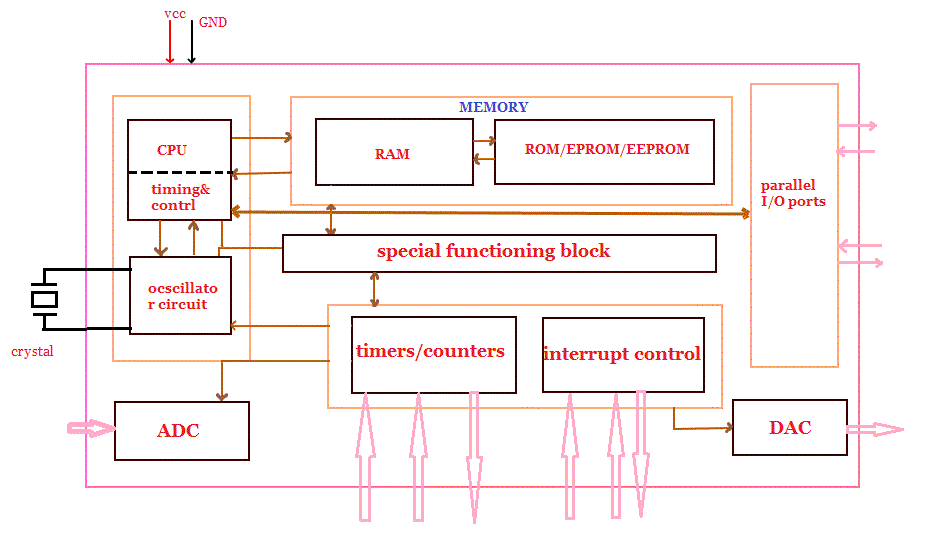
\includegraphics[scale=0.4]{images/mcudia.png}
	\caption{Microcontroller Block Diagram (taken from  \cite{mcudia})}
	\label{mcudia}
	\end{figure}
	\section{The Raspberry Pi}
	The Raspberry Pi is a small (85mm x56mm) \cite{pi3mechdraw} computer running a version ("flavour") of GNU/Linux called "Raspian" (although it is able to run a number of other operating systems depending on the situation (CITE). The first Raspberry Pi (Model A) had a single core 700MHz processor and 256MB of RMA \cite{pi1info}, while the current Raspberry Pi 3 Model B has a quad core 1.2GHz and 1GB of RAM (also including built in WiFi and Bluetooth) \cite{pi3info}. The quad core processor enables better multithreaded operation for software running on the Raspberry Pi, meaning that big cumbersome programs can run much more efficiently than before. In addition, the increase in memory and CPU clock frequency means there is overall a massive performance boost. Operations like compiling a large program (for example OpenCV, the Open Source Computer Vision Library) which would take over 9 hours \cite{pipowercompold} on the Raspberry Pi 1, take little over an hour and a half \cite{pipowercompnew} on the lastest model.\newline 
	\begin{figure}[h!]
	\centering
	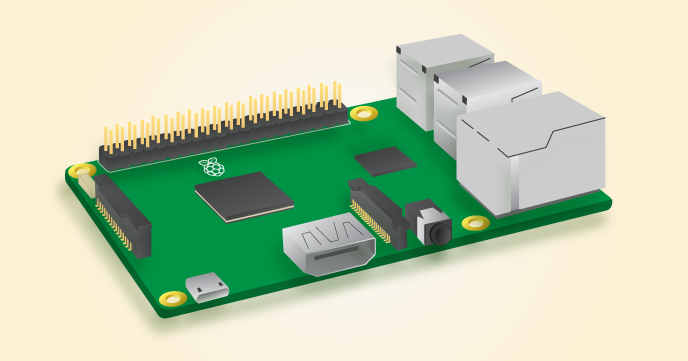
\includegraphics[scale=0.5]{images/pi3modelb.png}
	\caption{Raspberry Pi 3 Model B (taken from  \cite{pi3info})}
	\label{pidia}
	\footnotesize Clockwise from top left: GPIO pins, USB ports, Ethernet port, audio jack, camera module port, HDMI port, micro-USB power port, and LCD display port.
	\end{figure}
	\newline What makes the Raspberry Pi interesting, are the GPIO (General Purpose Input/Output, see Figure \ref{pidia}) pins made available on the main board. These pins allow electronic circuits to interface with the Raspberry Pi, and allows software to interact with the real world in a way that is not as easy to accomplish with a tradition computer. This marriage of PLC and PC allows for incredibly easy development and testing in a single package.
	%History
	%what is
	%what for
	\section{This Thesis}
	%Why use the Pi/What makes it suitable/How will it be used

	%\chapter*{Description of the Organisation}
	%\addcontentsline{toc}{chapter}{Description of the Organisation}
	%In this section, you should show a good understanding of the organisation. Details may include the type of organisation, management structure, products, and markets catered for. Mention your position in the organisation.
	
	\chapter*{Description of the Work}
	\addcontentsline{toc}{chapter}{Description of the Work}
	%Elaborate on issues mentioned in introduction. Use a logical development, not necessarily in chronological order. Explain the significance, purpose and nature of your work. Describe methods used and outcomes. Try to ensure a balanced treatment of issues, in accordance with their relative importance, and excluding irrelevant material. Present results and discuss around them. Explain the significance of these results and their impact on the organisation. Comment on technical difficulties you may have experienced. In a long report, subdivide with appropriate sub-headings, or divide this section into different sections. Equations should be numbered sequentially (see templates document).
	
	\chapter*{Conclusions}
	\addcontentsline{toc}{chapter}{Conclusions}
	%Summarise findings and inferences mentioned in the core of the report. Try to be as brief as possible, with concise statements. Include recommendations, where appropriate. 
	
	\chapter*{Review}
	\addcontentsline{toc}{chapter}{Review}
	%Relate this section to the learning objectives in the introduction. Report what you have learnt about the organisation and about yourself. Mention your achievements, what you have learnt, skills you have acquired or improved. This might be technical or "soft" skills. Try to relate this to what you have learned in your coursework at University and what skills you will take forward to your first full time professional post.
	
	\chapter*{Nomenclature}
	\addcontentsline{toc}{chapter}{Nomenclature}
	%List all the symbols in alphabetical order, with Greek symbols at the end.
	\begin{center}
		\begin{tabular}{|c|c|}
			\hline
			\rule{3cm}{0pt}\textbf{Symbol}\rule{3cm}{0pt} & \rule{3cm}{0pt}\textbf{Description}\rule{3cm}{0pt} \\
			\hline
			 & \\
			\hline
			& \\
			\hline
			& \\
			\hline
			& \\
			\hline
			& \\
			\hline
			& \\
			\hline
			& \\
			\hline
			& \\
			\hline
		\end{tabular}
	\end{center}
	
	%Bibliography
	\bibliography{biblio}
%	\bibliographystyle{apalike}
	\bibliographystyle{unsrt}
	
	%Appendix
	\chapter*{Appendix}
	\addcontentsline{toc}{chapter}{Appendix}
	\pagenumbering{alph}
	\setcounter{page}{1}
		
\end{document}